\subsection{Równanie geodezyjnej} %//w pobliżu czarnej dziury Schwarzschilda

%Po pierwsze zauważmy, że nie interesuje nas tak naprawdę samo $gamma$, gdyż ono opisuje tylko położenie w zależności od czasu. W naszym przypadku o wiele bardziej przydatna będzie znajomość wektora prędkości, czyli $frac(d gamma, d t)$, który tak naprawdę jest szczególnym przykładem pola wektorowego wzdłuż krzywej, czyli przyporządkowania 
%$ V:I arrow T"BH" $ 
%takiego, że dla dowolnego $t in I$ zachodzi $V(t) in T_(gamma(t))"BH"$. 
%
%//Rozważmy pokrycie rozmaitości $"BH"$ mapami $(bb(R) times (0, +oo) times U_i^plus.minus, phi_i^plus.minus)$, gdzie zbiory $U_1^+$ i $U_1^-$ to odpowiednio prawa i lewa półkula sfery $S^2$, natomiast $U_2^+$ i $U_2^-$ to górna i dolna półkula. Odwzorowania $phi_i^plus.minus$ to wówczas identyczność na pierwszych dwóch współrzędnych, a rzut na płaszczyznę $bb(R)^2$ z odpowiedniej półkuli. Wiemy, że funkcje $frac(diff, diff (phi_i^plus.minus)^j)$ są bazą przestrzeni stycznej w dowolnym punkcie mapy $phi_i^plus.minus$.]

Ponieważ foton nie przyśpiesza podróżując po przestrzeni wokół czarnej dziury, tzn. druga pochodna krzywej opisującej jego trasę jest stale równa zero, to mówimy, że trasa zataczana przez foton jest \textbf{linią geodezyjną} na rozmaitości $BH$. Linia geodezyjna jest najszybszą (najkrótszą) ścieżką między dwoma punktami - taką właśnie najmniej pochłaniającą energię drogę wybierają zazwyczaj obiekty fizyczne.

Zauważmy, że patrząc na podróż fotonu, przesuwamy wraz z nim przestrzeń styczną, zawierającą wektor prędkości, po krzywej którą ów foton zatacza. Patrząc znów na prosty przykład na $S^2$, przyjrzyjmy się co się dzieje z wektorami stycznymi kiedy przesuwamy je na dwa sposoby między tymi samymi punktami leżącymi na równiku, jak na rysunku \ref{rysunek sfera przestrzenie styczne}.

\begin{figure}[h]
  \centering 
  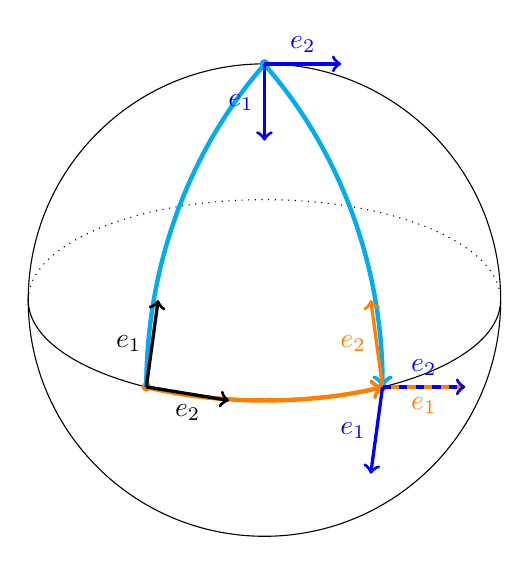
\begin{tikzpicture}
    \draw (0, 0) circle (3);
    \draw (-3, 0) arc (180:360:3 and 1.275);
    \draw[dotted] (-3, 0) arc (180:0:3 and 1.275);

    \draw[orange, ultra thick, ->] (0, -1.275) arc (270:300:3 and 1.275);
    \draw[orange, ultra thick] (0, -1.275) arc(270:240:3 and 1.275);

    \filldraw[orange] (-1.5, -1.1025) circle (1.5pt);
    \filldraw[orange] (1.5, -1.1025) circle (1.5pt);

    \draw[cyan, ultra thick] (-1.5, -1.1025) arc (180:135:5.25 and 5.85);
    \draw[cyan, ultra thick, <-] (1.5, -1.1025) arc (0:45:5.25 and 5.85);

    \filldraw[cyan] (0, 3) circle (1.5pt);

    \draw[->, very thick] (-1.5, -1.1025)--(-1.35, 0) node [midway, left] {$e_1$};
    \draw[->, very thick] (-1.5, -1.1025)--(-0.45, -1.275) node [midway, below] {$e_2$};

    \draw[->, very thick, blue] (0, 3)--(0.975, 3) node [midway, above] {$e_2$};
    \draw[->, very thick, blue] (0, 3)--(0, 2.025) node [midway, left] {$e_1$};

    \draw[->, very thick, orange] (1.5, -1.1025)--(1.35, 0) node [midway, left] {$e_2$};
    \draw[->, very thick, orange] (1.5, -1.1025)--(2.55, -1.1025) node [midway, below] {$e_1$};
    
    \draw[->, very thick, blue, dashed] (1.5, -1.1025)--(2.55, -1.1025) node [midway, above] {$e_2$};
    \draw[->, very thick, blue] (1.5, -1.1025)--(1.35, -2.205) node [midway, left] {$e_1$};
  \end{tikzpicture}
  \caption{Różnica między przestrzeniami stycznymi przesuwanymi po równiku a przestrzeniami stycznymi przesuwanymi po południkach.}\label{rysunek sfera przestrzenie styczne}
\end{figure}

Idąc przez północny biegun sfery wektory styczne obracają się i na końcu trasy nie zgadzają się z wektorami, które były przesuwane po równiku. Przesuwanie wektorów stycznych wzdłuż krzywej kryje w sobie składanie pól wektorowych - pola zawierającego wektory prędkości na krzywej i pola zawierającego wektory bazowe przestrzeni stycznej. W celu uzgodnienia tego, jak przesuwać przestrzeń styczną wzdłuż krzywej, lub bardziej ogólnie jak składać pola wektorowe, potrzebne jest użycie koneksji Levi-Civity, której dokładniejsza definicja znajduje się w {\color{red}dodatku}.

%\textbf{Koneksja Levi-Civity} jest połączeniem affinicznym, który składowe pola wektorowego przenosi na przestrzeń stycznyną nieskończnenie odległą od rozmaitości. Można o tym myśleć jako o rzutowaniu wektorów stycznych w różnych punktach na daleką kartkę papieru. Dzięki temu możemy porównywać pola wektorowe w dowolnych punktach na rozmaitości. 

%Formalna definicja koneksji Levi-Civity mówi, że jest to połączenie affiniczne $nabla$ które 
%- zachowuje metrykę, tzn. $nabla g=0$ 
%- oraz jest pozbawione torsji, tzn. dla dowolnych pól wektorowych $X, Y$ mamy $nabla_X Y-nabla_Y X=[X, Y]$, gdzie $[X, Y]$ jest pochodną Liego $X, Y$.
%

Jeśli teraz $x_1,..., x_n$ są lokalnymi współrzędnymi na rozmaitości, a $\partial_1,...,\partial_n$ wektorami bazowymi przestrzeni stycznej, to możemy zdefiniować \textbf{symbole Christoffela} dla koneksji $\nabla$ względem tego układu współrzędnych jako liczby spełniające poniższą równość:
$$ \nabla_j \partial_k=\Gamma_{j k}^l \partial_l. $$
W przypadku czarnej dziury rolę koneksji Levi-Civity będzie spełniać pochodna względem czasu właściwego $\frac{d}{d\tau}$. W celu uproszczenia notacji i zadowoleniu zmysłu konformizmu z popularną notacją, dla wektora $v$ będziemy pisać 
$$ \nabla v = \frac{d}{d\tau} v = \dot{v}. $$

Niech więc $x_i$ będzie lokalnym układem współrzędnych na $BH$. Wtedy krzywa $\gamma$ zadaje gładkie funkcje $t \mapsto x_i (t)=x_i (\gamma(t))$, które dają funkcję $\R \to \R^4$. W celu uproszczenia notacji będziemy 
od razu pisać $x_i=x_i(t)$. Równanie różniczkowe opisujące geodezyjną którą podróżuje foton przedstawia się wtedy jako
%//$ nabla accent(gamma, dot) (t) = Gamma_(i,j)^k (x_1(t),...,x_4(t))frac(d x^i, d t) frac(d x^j, d t) = 0 $
$$ \ddot{\gamma} = - \Gamma_{i,j}^k \dot{x^i} \dot{x^j} $$
gdzie $\Gamma_{i,j}^k$ to symbol Christoffela drugiego rodzaju.%//, natomiast $dot$ nad zmienną oznacza branie jej pochodnej względem pewnej affinicznej parametryzacji, która przychodzi razem z koneksją Levi-Civity.

Dodatkowo, ponieważ foton jest cząsteczką bez masy, geodezyjna którą on podróżuje jest określana \emph{nullową} geodezyjną i musi spełniać dodatkowy warunek
$$ g_{\mu,\nu} \dot{x^\mu} \dot{x^\nu} = 0 $$
gdzie $g_{\mu,\nu}$ to wartość tensora metrycznego $g(\mu, \nu)$.








%//wyznaczony za pomocą koneksji Levi-Cevity. W szczególności interesuje nas fakt, że $i$-ta współrzędna wektora prędkości fotonu wyraża się jako
%//$ gamma ^i (t)= -Gamma_(m,j)^i frac(d x^m, d t) gamma ^j (t). $
%
%/*Symbole Christoffela użyte w obliczeniach zostały zaczerpnięte z @symboleGotowe.
%
%Ponieważ foton w naszym przypadku porusza się po płaszczyźnie przechodzącej przez równik, to $x^3 = theta = pi / 2$ jest funkcją stałą. Interesują nas więc tylko wartości zmiany $phi=x^4$ oraz $r=x^2$ w czasie, czyli
%/*$ phi' = -( 1 / r r' phi + 1 / r phi' r)=-( phi / r r' + phi') $
%$ r' = - ( frac(G M, r^2) (1 - (2G M) / r ) t - frac(G M, r^2) (1 - (2G M) / r)^(-1) r' r ) $ */
%
%$ phi' =  -Gamma_(r, phi)^phi r' phi - Gamma_(theta, phi)^phi theta' phi=- frac(r', r) phi - 0 $
%$ r' = -Gamma_(t, t)^r t' t - Gamma_(phi, phi)^r phi' phi -Gamma_(theta, theta)^r theta' theta - Gamma_(r, r)^r r' r = -e^(2 X - 2 V) frac(diff_r X, diff r) t + r e^(-2 V)phi' phi - frac(diff V, diff r) r' r $
%
%gdzie
%$ e^(2x)= e^(-2V)=(1- frac(2G M, c^2 r)) $
%
%Czyli równanie to 
%$ phi' = -frac(r', r) phi $
%$ r' =  $
%*/
%
